\documentclass[twocolumn,11pt]{article}
\usepackage{10x23project}

\begin{document}

\title{Generating Urban Massing in Context from Text and Block Graphs}
\author{Daehong Kim \& James Fu \& Chenyue Shen\\
\texttt{\{daehongk, jfu2, chenyues\}@andrew.cmu.edu}\\
10-x23 Generative AI Course Project}
\date{\today}
\maketitle

% \linenumbers

\begin{abstract}
In early urban design, density, height and use are set for each block before any building is drawn. Given a map of a real neighborhood with a few blocks left empty and one sentence about them, we generate a 2.5D map of buildings for the empty blocks that meets such per-block targets. A language model turns the sentence into these targets, and a graph-conditioned discrete diffusion model adapted from \citet{liu2025controllable} generates the map. We use NYC open data and compare against the original Liu model and GlobalMapper \citep{he2023globalmapper}.
\end{abstract}


\section{Introduction}
When designers plan new buildings for a few city blocks, they first fix coverage, floor area ratio (FAR), height and use per block, the terms zoning codes use, and then try massings that meet these numbers and fit the site. Many layouts meet the same numbers, so this step suits a generative model that draws several layouts for one condition.

Existing models cover parts of this step. Some learn realistic layouts from real cities without user control \citep{he2023globalmapper,he2024coho}, some take density targets for a single site \citep{zhuang2024texttocity,gao2025genfusion}, and \citet{liu2025controllable} control 3D outdoor scenes with a scene graph of objects in synthetic driving scenes. We bring these together for real city blocks: a language model turns a short request into target numbers per block, which the user can read and edit, and a modified version of the model of \citet{liu2025controllable} fills the masked blocks from a graph of all blocks in the map (Figure~\ref{fig:overview}). We use official NYC records and compare against the original Liu model and a replicated GlobalMapper on held-out districts.

Our key contribution is a novel application of an existing method \citep{liu2025controllable} to a new task, with three changes to its architecture. We will deliver a block-level NYC dataset, measure what each change does, and split the remaining error between the language and generation steps.

\begin{figure*}[t]
    \centering
    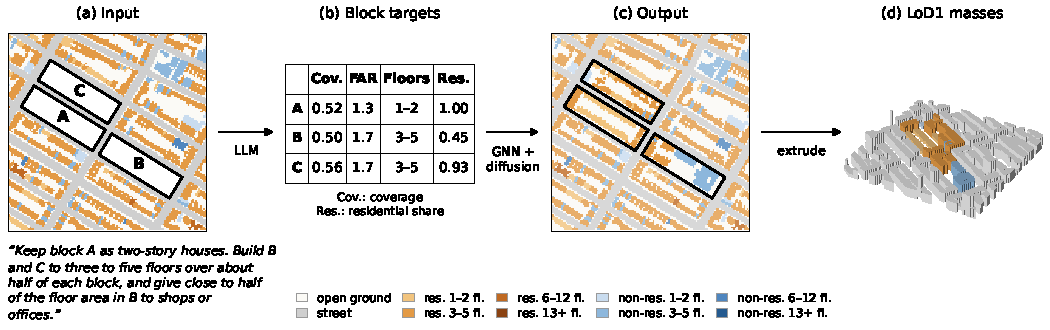
\includegraphics[width=\textwidth]{fig/overview.pdf}
    \caption{One real sample from Park Slope, Brooklyn: (a) 512\,m tile with three masked blocks and a request, (b) targets from the language model, (c) blocks filled by the diffusion model (shown: the real map, i.e.\ the training target), (d) extrusion.}
    \label{fig:overview}
\end{figure*}


\section{Dataset / Task}
\paragraph{Data.} We use three NYC open datasets: PLUTO\footnote{\url{https://data.cityofnewyork.us/d/64uk-42ks}} (land use, floors and FAR per tax lot), Building Footprints\footnote{\url{https://data.cityofnewyork.us/d/5zhs-2jue}} (outlines and roof heights) and Tax Lots\footnote{\url{https://data.cityofnewyork.us/d/i38t-6if2}} (lot boundaries). We chose NYC because its blocks, heights and floor counts come from official city records, and the city publishes them without restrictions on use. We build on the released code of \citet{liu2025controllable}\footnote{\url{https://github.com/yuhengliu02/control-3d-scene}} and of GlobalMapper\footnote{\url{https://github.com/Arking1995/GlobalMapper}}.

Merging tax lots by block number gives official block polygons, space outside lots is street, and for each block we compute coverage, FAR, median floors and residential share. Around each group of target blocks we cut a 512\,m tile and rasterize it at 4\,m into a $128\times128$ map with 10 classes: street, open ground, and residential or non-residential buildings in four height classes (1--2, 3--5, 6--12, 13+ floors). In a test on Park Slope, 94\% of footprints linked to a PLUTO lot, and block FAR from footprints matched PLUTO records with a correlation of 0.88. A target group is 1 to 4 adjacent blocks, so each block appears in several samples. NYC has about 28,800 blocks, which we split by community district so that test neighborhoods are unseen.

No text is written or labeled by hand. An LLM writes requests from true block tables in varied styles (exact numbers, words such as ``dense'', comparisons with neighbors). Vague words are tied to NYC quantiles; for example, ``dense'' means the top third of block FAR. We keep the requests from which a second LLM pass recovers the table.

\paragraph{Task.} Let $x$ be the class map of a tile, $M$ the mask of 1 to 4 target blocks, $\mathcal{B}$ the block polygons and $s$ the request. A language model gives a target table $T = f(s, \mathcal{B}, x_{\bar M})$, and the generator samples
\begin{equation}
    \hat{x}_M \sim p_\theta\left(x_M \mid x_{\bar M}, M, \mathcal{B}, T\right).
\end{equation}
The map outside $M$ is fixed, and samples for one input should differ while still meeting $T$. The generator is trained with true tables and tested with parsed ones.

\paragraph{Metrics.} Condition error is the per-block error in coverage and FAR and the accuracy of height class and dominant use. Fit with the surroundings is the share of building cells on the street (Out-Block in \citet{he2023globalmapper}) and how close height differences across the mask boundary are to real tiles. Realism is the accuracy of a small CNN trained to separate real and generated target regions (50\% is best) and the distance between distributions of footprint measures such as building size and spacing \citep{fleischmann2019momepy}, computed on polygons traced from connected building cells of generated and real blocks. Diversity is the share of cells that differ between four samples drawn for one input. We report means over test blocks with 95\% bootstrap intervals.


\section{Related Work}
Scene-graph conditioning began with images \citep{johnson2018sg2im}. \citet{liu2025controllable} bring it to 3D outdoor scenes with a graph attention network \citep{velickovic2018gat}, a module that places nodes on a bird's-eye-view grid, and discrete diffusion \citep{austin2021d3pm}. They also turn text into the graph with an LLM, as our request step does. Their nodes are objects in synthetic driving scenes whose positions must be learned, while in a city the block outlines are known.

Learning-based urban layout generation began with single blocks. BlockPlanner \citep{xu2021blockplanner} and GlobalMapper \citep{he2023globalmapper} generate the buildings of one block from its shape with graph-based models, so neighboring blocks can look unrelated. COHO \citep{he2024coho} generates whole cities with heights, and CityDreamer \citep{xie2024citydreamer} generates unbounded semantic and height maps. None of them lets a user set the density or use of a block.

Work in architecture and planning adds design targets. Text-to-City \citep{zhuang2024texttocity} conditions Stable Diffusion on a density token and fails when several indicators are given together. GenFusion \citep{gao2025genfusion} conditions diffusion on FAR and building density for one site. \citet{jang2026context} inpaint one site's footprint from its roads and neighbors without density targets, and CoMa \citep{maslov2026coma} generates one parcel's massing from its context with a vision-language model. Our task combines what these works do separately: several blocks at once, inside a real context, each with its own numeric targets, through a table the user can edit.


\section{Approach}
\paragraph{Request to table.} A prompted LLM (Qwen3-8B, no training, a few examples from training districts in the prompt) reads the request with the target blocks and the true values of the surrounding blocks, and returns a JSON table of coverage, FAR, height class and residential share per target block.

\paragraph{Table to map.} In the 2D stage of \citet{liu2025controllable}, a GNN and an allocation module build a bird's-eye-view embedding map that conditions a jointly trained discrete diffusion model. This suits our task: the graph keeps each target attached to its block and lets neighboring blocks inform each other, and discrete diffusion models a categorical map and gives several samples for one condition. Applied to our data as is, each block becomes a node with only a class label (dominant use and height class) and an approximate center, the allocation module learns where to place it, and the model generates the whole tile without context, which we evaluate inside the mask. We change this in three steps. First, each node gets the four target values and its area as numeric attributes (true values for surrounding blocks, the table for target blocks), and blocks facing each other across a street are connected. Second, instead of learning a position, we write each node embedding into every cell of its known polygon, and street cells get one learned embedding. Third, the diffusion model receives the real map outside the mask and the mask as extra channels, and noise and loss apply only inside the mask. We otherwise keep Liu's network, noise schedule and training settings. Cells are then extruded by height class, replacing Liu's 3D stage.

Our key contribution is therefore a novel application of an existing method to a new task, with these three architectural changes.

\paragraph{Baselines and replication.} The original Liu model above is our first baseline. Its training graphs and weights are not released, so its own numbers cannot be replicated. GlobalMapper is our second baseline and our replication target. Its full 120K-block dataset needs a Purdue sign-in and its repository has no evaluation code, so we will train on the released 10K-block sample, implement its metrics from the paper, ask the authors for the full data, and report our numbers next to the published ones (L-Sim 22.45, Overlap 1.42\%, Out-Block 0.89\%, FID 14.94). Retrained on NYC, its output is rasterized to our grid and compared on footprint realism, Out-Block and continuity, since it has no heights or targets.


\section{Expected Outcomes}
Our research question is whether a scene-graph diffusion model can meet numeric targets for several blocks at once while staying consistent with a real neighborhood, and which part of the pipeline limits it. We train five models on the training districts and test them on held-out districts: the original Liu model, the model after each of our three changes, and GlobalMapper. Running the generator with the true table instead of the parsed one splits the error between the two steps. We expect that:

\begin{enumerate}
    \item Numeric attributes lower per-block FAR and coverage error, since the original graph cannot express density.
    \item Area allocation lowers these errors further and reduces Out-Block, since the model no longer has to infer where each block is.
    \item The context input brings height differences across the mask boundary closer to real tiles, and the final model is close to GlobalMapper on footprint realism but more continuous across block edges, since GlobalMapper sees one block at a time.
    \item Most remaining condition error comes from the generation step, because meeting several numbers at once inside a fixed context is harder than filling a table from a short request.
\end{enumerate}

The results also tell us where to put effort. If numeric attributes alone remove most of the error, the known block outline matters less than we expect. If parsed tables cause most of the error, the request format needs more work than the generator. Because every request is written by an LLM, our results do not show how the pipeline handles the way real users phrase requests.


\section{Plan, Human Work and AI Use}
\paragraph{Work split.} Daehong Kim builds the NYC pipeline and evaluation code, James Fu trains the original Liu model and implements the three changes, and Chenyue Shen builds the request generation and LLM step and runs GlobalMapper. Daehong and James pair-program the area allocation and context input, which touch both the data and the model.

\paragraph{Milestones.} Nov 7--11 (liaison): confirm the replication plan. Nov 14: NYC dataset complete; GlobalMapper training on its sample. Nov 20 (midway): GlobalMapper replication table, first NYC results of the original Liu model, evaluation code, request generation. Nov 27: three changes trained; LLM step evaluated. Dec 1: GlobalMapper on NYC; full comparison. Dec 4 and 10: poster, final summary and code. Each model fits on one 24\,GB GPU.

\paragraph{Risks.} The code of \citet{liu2025controllable} is built for 3D scenes, so we first cut it down to the 2D stage and check that it can overfit a few NYC tiles before full training. If the five models do not fit in time, we drop the NYC retraining of GlobalMapper and keep its replication. If Qwen3-8B parses requests poorly, we switch to a larger model, which changes only the first step.

\paragraph{Human work and AI use.} The team decides the task, data, model changes and experiments, checks the pipeline against PLUTO records, and writes the analysis. Each week we also read a random set of generated requests and maps to catch failures the metrics miss. We expect to use AI coding assistants such as Claude Code for data and evaluation scripts, which we review and test against known values. LLMs are also part of the method, where they write and parse requests.


\bibliographystyle{plainnat}
\bibliography{references}

\end{document}
